
\section{Introdução}
CE20211 é o nome provisório do modelo de simulação que será desenvolvido de forma conjunta pela turma, para a realização de experimentos didáticos no âmbito da disciplina-turma Computação Experimental, no semestre 2021.1

Este capítulo apresenta uma descrição padronizada do modelo, adotando-se o protocolo ODD \citep{grimm_standard_2006}.

Para suporte e detalhamento, ver os slides em \ref{oddprotocol}, juntamente com as aulas gravadas.

\section{Overview}

\subsection{Propósito do Modelo - Geral}\label{sec:proposito}

\begin{quote}
    Descreva aqui o propósito do modelo de simulação do processo de produção científica no domínio de simulação multiagente de sociedades.
\end{quote}

O propósito do modelo de simulação será auxiliar na compreensão de como o comportamento social dos cientistas (seres humanos) – em particular:
\begin{itemize}
    \item 
envolvimento em projetos de pesquisa científica como investigadores \footnote{
Um projeto científico é um empreendimento temporário, executado com recursos limitados, com participação de cientistas, aspirantes a cientistas, técnicos - que tem por objetivo produzir algo novo (no caso, um novo conjunto de conhecimentos científicos – dados, relatórios, artigos, publicações)}
\item filiação a Organizações, a \replaced[id==JHCF]{Territórios}{países}, 
\item atuação em áreas das ciências humanas ou naturais, ou culturais ou tecnológicas, 
\end{itemize}

afeta o seu desempenho, em particular a produtividade científica (dos cientistas), mensurada por índices de impacto, tais como:
\begin{itemize}
\item Índice H
\item Índice G
\item outros 
\end{itemize}


Exercício 3.2: 2 pontos: Contribua com entre 20 e 50 palavras em complementação ao propósito do modelo declarado acima, segundo a ideia de declaração de propósito descrita no protocolo ODD \citep{grimm_standard_2006}.
Na sua contribuição, faça referência a pelo menos uma fonte de informação na Internet, usando uma URL ou referência no Zotero.

\subsubsection{Complementação ao propósito do Modelo segundo aluno Guilherme Mendel}
Acredito que talvez seja interessante observar como esses fenômenos sociais influenciam cientistas de diferentes \href{https://pt.wikipedia.org/wiki/Gera\%C3\%A7\%C3\%A3o}{gerações} ou territórios. Cientistas ativos no século 20 podem apresentar resultados diferentes dos cientistas ativos atualmente, por exemplo.

    
\subsubsection{Complementação ao propósito do Modelo segundo aluna Jaqueline Gutierri Coelho}
Minha complementação ao propósito do modelo trata-se da discrepância de métodos científicos(experimentações científicas) utilizados por cada cientista, pois cada cientista possui a intervenção dos meios em que foi criado, e do local onde foi realizado seus estudos em sua formação. \citep{vernotte_risk-driven_2015}

\subsubsection{Complementação ao propósito do Modelo segundo aluna Caroline Ferreira Pinto}
Complemento o propósito do modelo descrito anteriormente dizendo que, além dos fatores citados acima, a história de vida de um cientista também interfere em suas pesquisas, já que cada um deles possui uma preferência em relação à áreas de estudo ou uma familiaridade com certo assunto. \href{https://comportese.com/2014/05/01/o-comportamento-do-cientista}{Fonte}

\subsubsection{Complementação ao propósito do Modelo segundo aluno Otávio Souza de Oliveira}

Complementando o modelo, um dos principais aspectos que mobilizam um pesquisador na produção científica é a \href{https://www.scielo.br/j/pci/a/ww5zR3KhYCk65bPkWJyTQtf/?lang=pt}{internet} que facilita nas pesquisas, referências, na busca por informações. Mas por sua vez com a quantidade enorme de informações já divulgadas, podem atrapalhar o crescimento desse pesquisador no quesito reconhecimento e assim desmotivá-lo.

\subsubsection{Complementação ao propósito do Modelo segundo aluna Kailany Ketulhe Gomes Rocha}

A minha complementação ao modelo descrito na seção \ref{sec:proposito}, seria entender os recursos disponíveis e utilizados pelos cientistas nas suas produções, entendendo as limitações de suas pesquisas. A escassez de
\href{https://conexao.ufrj.br/2019/02/escassez-de-verbas-corroi-pesquisa-cientifica-nacional/}{recurso} pode influenciar no desenvolvimento de uma pesquisa e na manutenção da mesma.

\subsubsection{Complementação ao propósito do Modelo segundo o aluno Álvaro Veloso Cavalcanti Luz}

Como complementação para o modelo, é importante que sejam notados aspectos que afetam a produtividade científica. Por exemplo, um desses aspectos é a inconsistência do apoio financeiro à área, visto que os investimentos públicos para pesquisa são constantemente alvos de \href{https://www.redebrasilatual.com.br/educacao/2021/04/educacao-e-a-area-mais-atingida-pelos-cortes-orcamentarios-de-bolsonaro/} {cortes e imposições de tetos de gastos} no Brasil atual.

\subsubsection{Complementação ao propósito do Modelo segundo aluna Giovana Pinho Garcia}
Algo muito importante que afeta a produtividade de um cientista é o financiamento por parte do governo ou de algum patrocinador. Essa falta de financiamento pode afetar muito o desempenho de cientistas principalmente de baixa renda. \href{https://www.ufg.br/n/129177-baixo-investimento-em-ciencia-e-tecnologia-eleva-a-desigualdade-social}{Fonte}.

\subsubsection{Complementação ao propósito do Modelo segundo aluno Vitor Vasconcelos de Oliveira}
Um fato válido e importante para o modelo retratar, seria o aspecto do acesso à educação no ambiente de criação dos cientistas. Muitos lugares no mundo não proporcionam um acesso adequado a educação e ao conhecimento, isso pode gerar discrepância na forma que o conhecimento científico é dividido pelo mundo.
\href{https://www.senado.gov.br/noticias/Jornal/emdiscussao/inovacao/pesquisa-ciencia-tecnologia-e-inovacao-educacao/caminho-para-o-conhecimento-cientifico-e-a-inovacao-tecnologica-no-pais-ensino-de-ciencias-nas-escolas-e-desafio-para-alunos-e-professores-do-brasil.aspx}{Fonte}

\subsubsection{Complementação ao propósito do Modelo segundo aluno Leonardo Rodrigues de Souza}
Como complementação para o modelo, é importante entender como sustentar áreas da ciência que não trazem um grande retorno financeiro ao mercado, já que esse tipo de pesquisa costumam trabalhar escassez de recursos, ou mesmo serem cortadas rapidamente. \href{https://exame.com/ciencia/crise-na-ciencia-nao-se-deve-so-a-falta-de-recursos/}{Fonte}

\subsubsection{Complementação ao propósito do Modelo segundo aluno Rafael Gonçalves de Paulo}
A capacidade produtiva de um pesquisador depende da sua qualidade de vida, que, pelo pesquisador estar inserido num ambiente político e social, depende das políticas públicas de onde vive. Incorporar essa lógica no modelo pode ser interessante como complementação ao modelo. \href{https://www.revista.ueg.br/index.php/mirante/article/view/7103}{Fonte}.

\subsubsection{Complementação ao propósito do Modelo segundo aluno João Gabriel Ferreira Saraiva}
Uma coisa que ocorre muito no nosso país, é a falta de conhecimento das pessoas sobre os trabalhos científicos desenvolvidos, principalmente nas universidades, é um desses desafios, o que faz com que os impactos gerados por essas pesquisas não sejam de conhecimento da população. \href{https://www.periodicosdeminas.ufmg.br/entenda-os-atuais-desafios-das-pesquisas-cientificas/}{Fonte}

\subsubsection{Complementação ao propósito do Modelo segundo aluno João Pedro Sadéri da Silva}
Para a complementação desse modelo, a falta de matérias adequados e a ausência de infraestrutura para o \href{https://www.blogs.unicamp.br/socialmente/2011/08/23/o-que-e-e-para-que-serve-um-experimento/}{experimento} pode gerar impacto na forma como é obtido resultados dessa pesquisa.

\subsubsection{Complementação ao propósito do Modelo segundo aluno Lucas Vinicius Magalhães Pinheiro}
Um outro fator que impacta na produção científica de cientistas é a questão financeira. Mais em foco, no âmbito de quais tópicos agregam interesse de investidores, tendo assim um agregado de tópicos que angariam mais atenção. Assim, a liberdade criativa do pesquisador é limitada pelo potencial financeiro de sua pesquisa. \href{https://revistapesquisa.fapesp.br/conflito-de-interesses-um-desafio-inevitavel/}{Fonte}

\subsubsection{Complementação ao propósito do Modelo segundo aluno Thales Lima Menezes}

Visando complementar o propósito do modelo sugerido acima proponho avaliar a presença em redes sociais dos cientistas; o objetivo é observar a habilidade dos cientistas em compartilhar o conteúdo de suas pesquisas com a população não acadêmica, podendo incluir contato com possíveis investidores. \href{https://vejasp.abril.com.br/cultura-lazer/influencers-ciencia-atila-iamarino/}{Fonte}

\subsubsection{Complementação ao propósito do Modelo segundo aluno Heitor de Lima Belém}https://pt.overleaf.com/project/60f1998bd62a4772843288a0
Para complementar o modelo, é necessário avaliar aspectos que afetem a produtividade científica. A proximidade da sociedade com as universidades é um deles. Com o apoio social, é mais provável que mais investimentos sejam feitos na área de produção científica de modo que haja maior desenvolvimento e engajamento em pesquisas. \href{https://www.periodicosdeminas.ufmg.br/entenda-os-atuais-desafios-das-pesquisas-cientificas/}{Fonte}

\subsubsection{Complementação ao propósito do Modelo segundo aluno João Francisco Gomes Targino}
Como um dos fatores que impacta na produção científica, o desequilíbrio de gênero é um deles, pois a hegemonia masculina prevalece nos ganhos de verbas e bolsas, essa discrepância acontece em quase todas as áreas mas principalmente na de Engenharia, Ciências Exatas e da Terra.
\href{https://sites.usp.br/psicousp/desequilibrio-de-genero-afeta-mulheres-cientistas-brasil/}{Fonte}

\subsubsection{Complementação ao propósito do Modelo segundo aluno João Victor Pinheiro de Souza}

Um dos autores que influência a produção científica é a descrença na ciência, onde notícias falsa e teorias da conspiração são propagada com muita velocidade pelas redes sociais, o conhecimento científico virou alvo frequente de ataques de grupos de crenças, interesse politico e econômicos contrariados.
\href{https://revistapesquisa.fapesp.br/resistencia-a-ciencia/}{Fonte}

\subsubsection{Complementação ao propósito do Modelo segundo aluno Matheus Arruda Aguiar}

É importante ressaltar que fenômenos educacionais impactam consideravelmente na produção cientifica, dado que cada instituição de ensino é direcionada na visão pedagógica dos coordenadores e não uma instrução teórica, crítica despertando o interesse cientifico. \href{https://monografias.brasilescola.uol.com.br/pedagogia/influencia-globalizacao-praticas-educativas-e-reformulacao-conteudos.htm}{Fonte-Contemplação}

\subsubsection{Complementação ao propósito do Modelo segundo aluno Felipe Gomes Paradas}

Um dos fatores que mais impactam na produção científica é a jornada dupla para mulheres, enquanto cientistas ainda precisam prestar o papel de donas de casa e mães, o que afeta diretamente a produtividade. \url{https://agenciabrasil.ebc.com.br/radioagencia-nacional/economia/audio/2021-03/dupla-jornada-e-salarios-menores-realidade-que-ainda-afeta-mulheres}

\subsubsection{Complementação ao propósito do Modelo segundo aluno José Fortes Neto}

O modelo poderia ser complementado estudando os fatores externos que influenciam na qualidade da pesquisa, principalmente fatores atrelados ao apoio da sociedade aos trabalhos científicos e como eles são vistos. \href{https://www.periodicosdeminas.ufmg.br/entenda-os-atuais-desafios-das-pesquisas-cientificas/}{Fonte}


\subsubsection{Complementação ao propósito do Modelo segundo aluno Adelson Jhonata Silva de Sousa}
O propósito do modelo proposto pode ser complementando procurando entender os fatores que levam a fuga dos cérebros brasileiros, ou seja, a fuga dos pesquisadores brasileiros para continuar e terminar as suas pesquisas em outros países. \href{https://www.bbc.com/portuguese/brasil-51110626}{Fonte}


\subsubsection{Complementação ao propósito do Modelo segundo aluno João Gabriel Lima Neves}

O modelo poderia ser complementado fazendo uma analise de como aspectos burocráticos no processo de realização de pesquisas por profissionais afetam a suas pesquisas e a praticidade delas. Obstáculos existentes no processo de pesquisa em campo, que pressupõe uma articulação constante entre teoria e pratica, podem dificultar a utilização dos resultados dessas pesquisas.\href{https://www.scielo.br/j/icse/a/pZ8djC8vGSWbkQzwmKr4ByH/?lang=pt}{Fonte} 



\subsubsection{Complementação ao propósito do Modelo segundo aluna Alice da Silva de Lima}
Em complemento, uma vez que o presente trabalho está sendo realizado em um período pandêmico (COVID-19), o modelo também deve auxiliar na análise do número publicações do ano de 2020 em comparação aos anos anteriores, verificar se existe alguma anormalidade, isto é, um \href{https://medium.com/ensina-ai/outlier-o-ponto-fora-da-curva-1f28f3d9c23}{outlier} nessa métrica. É interessante observar essa questão geograficamente.

\subsubsection{Complementação ao propósito do Modelo segundo aluno Carlos Eduardo de Oliveira Ribeiro}
Um dos aspectos que pode ser observado tanto para o incentivo quanto para a desmotivação de uma produção científica é a existência da \href{https://pt.wikipedia.org/wiki/Pseudoci\%C3\%AAncia}{pseudociência} sobre um determinado assunto. A desmotivação por não conseguir o alcance como o de uma \textit{fake news} e incentivo para refutar aquilo que está circulando sem embasamento científico.

\subsubsection{Complementação ao propósito do Modelo segundo aluno Henrique Mendes de Freitas Mariano}
O modelo poderia cobrir sobre como a psicologia dos indivíduos que produzem ciência afeta na produção cientifica, pois dependendo do estado da psicologia do cientista sua produção pode ser afetada, assim diminuindo a sua contribuição para a ciência. \href{https://www.scielo.br/j/psoc/a/6X46nvFMKpmcLKv7HnYx76R/?lang=pt}{Fonte}.


\subsubsection{Complementação ao propósito do Modelo segundo o aluno Luthiery Costa Cavalcante}
Seria interessante ao propósito do modelo considerar como a presença massiva de determinado setor da indústria/comércio em uma cidade, região ou país, pode afetar o investimento e a produção científica dos indivíduos dessa localidade. \href{https://www.scielo.br/j/ss/a/FgDGxNb9L74g4fMch8kqM5F/?lang=pt}{Este artigo} aborda especificamente influências negativas da indústria na ciência local.

\subsubsection{Complementação ao propósito do Modelo segundo o aluno Gabriel Nazareno Halabi}
Um aspecto a ser observado como complemento ao modelo seriam as diferenças que se encontra entre o financiamento público e privado no desenvolvimento de produções científicas, considerando que há grandes diferenças no foco de investimento em diferentes países. \href{https://www.scielo.br/j/ep/a/WgdZnSMrX49LLTJMffmsqNK/?lang=pt}{Fonte}

\subsubsection{Complementação ao propósito do Modelo segundo aluno Paulo Maurício Costa Lopes}
Em complemento ao protocolo ODD seria interessante fazer um estudo das expectativas dos pesquisadores antes e depois do desenvolvimento de produções cientificas como também o senso critico deles antes e pós produção cientifica, \href{ https://noticias.unb.br/publicacoes/67-ensino/1938-iniciacao-cientifica-da-unb-e-premiada}{Texto exemplo}. 


\subsection{Redeclaração do propósito do modelo, após contribuições da turma}\label{sec:proposito:contrib}

\begin{quote}
    Segue nova descrição do propósito do modelo de simulação do processo de produção científica no domínio de simulação multiagente de sociedades, incorporando contribuições da turma, com acréscimos, esclarecimentos etc.
\end{quote}

O propósito do modelo de simulação será auxiliar na compreensão de como o comportamento dos cientistas 
é afetado por fatores diversos de ordem geral, como: 
\begin{itemize}
    \item Humana/Psicológica (pessoas que tem um ciclo/história de vida de nascimento, estudo acadêmico, ingresso, atividade e saída da carreira científica, experimentam infância, juventude, maturidade, envelhecimento, formação de família, filhos, tem aspirações geracionais, evolução da moral,  cognição\cite{sprouts_kohlberg_2019}, competitividade etc);
    \item Geográfica (clima, barreiras físicas-geográficas, vias de ligação terrestre, aérea, marítima com outros territórios etc, formando uma malha - grafo - com suporte a determinados tipos de fluxos de matéria, energia, pessoas e informação) etc;
    \item Cultural (tudo o que determina o comportamento coletivo, hábitos coletivos, sistema de valores e princípios coletivos, sistemas filosóficos, educação científica, tecnológica,  cultural e artística, integração com outros povos, isolamento cultural, equilíbrio de papéis e protagonismo entre gêneros, ausência de discriminação racial, étnica, sectarismo, multiculturalismo, multilinguísmo/plurilinguísmo,  visibilidade social dos cientistas, valorização do conhecimento científico versus o conhecimento dogmático/mitológico/religioso, de carreira acadêmica, valorização de pesquisa na indústria, comércio e serviços, atuação em determinadas estruturas sociais, em redes etc); 
    \item Histórica (fatos de alto impacto social e eventual permanência que determinam o curso/estágios de evolução do comportamento coletivo/cultural, experiência em conflitos, guerras, pandemias, apego a tradições etc); 
    \item Econômica (domínio do território na economia mundial, financiamento, investimentos e recursos para pesquisa, vida acadêmica, trabalho, integração com mercado, indução de \textit{startups}, equilíbrio de oportunidades entre territórios, empreendedorismo, simplicidade e agilidade no uso de recursos públicos etc); e
    \item Tecnológica (acesso a recursos e ferramentas, ambientes e infraestruturas de pesquisa e suporte à convivência acadêmica);
\end{itemize} 
e em particular:
\begin{itemize}
    \item 
envolvimento dos cientistas em projetos de pesquisa científica como investigadores \footnote{
Um projeto científico é um empreendimento temporário, executado com recursos limitados, com participação de cientistas, aspirantes a cientistas, técnicos - que tem por objetivo produzir algo novo (no caso, um novo conjunto de conhecimentos científicos – dados, relatórios, artigos, publicações)}, por meio de 
\item filiação a Organizações;
\item atuação em  \replaced[id==JHCF]{Territórios}{países}, 
\item pesquisa em áreas das ciências humanas ou naturais, exatas, ou tecnológicas, ou culturais;
\end{itemize}

afetando a produção de dados, relatórios, artigos científicos que resultam em publicações que permitem mensurar o desempenho individual, em particular a produtividade científica (dos cientistas), usando-se índices de impacto, tais como:
\begin{itemize}
\item Índice H
\item Índice G
\item outros 
\end{itemize}


\section{Variáveis de estado}

A partir de \citet{grimm_standard_2006}, as variáveis de estado podem ser elicitadas a partir de respostas às seguintes perguntas:
\begin{itemize}
\item ``What is the structure of the model system?'' 
\item ``For example, what kind of low-level entities (e.g., individuals, habitat units) are described in the model?'' 
\item ``How are they described?'' 
\item ``What hierarchical levels exist?'' 
\item ``How are the abiotic and biotic environments described?'' 
\item  ``What is the temporal and spatial resolution and extent of the model system?''
\end{itemize}

O modelo, a princípio, será composto por quatro níveis hierárquicos:
\begin{description}
    \item [Cientistas] agente representando as pessoas que realizam produção científica;
    \item [Organizações Cientificas] agrega agentes de vários tipos, representando as entidades que promovem e organizam a produção científica;
    \item [Territórios] agrega os agentes que representam os locais geográficos e onde a sociedade abriga as organizações e os cientistas;
    \item [Consumidores da Ciência Mundial] agrega os agentes que consomem o que é produzido pela ciência em alcance mundial;  
\end{description}

Cada um dos agentes nesses níveis é apresentado e detalhado a seguir.

\subsection{Nível dos Cientistas}

\subsubsection{Agente Cientista}
Apenas os agentes do tipo cientista compõem esse nível. 
Um agente cientista é um indivíduo, cientista, pesquisador etc, caracterizado por:
    \begin{description}
        \item [número de identificação] Ter uma identificação única na vida real, definida pelo ORCID ou similar. 
        \item [idade] ter uma idade em anos, que o caracteriza em um estágio da vida.
        \item [sexo] Ter um sexo, que em uma estrutura dominante machista, pode determinar certas limitações à atividade da pesquisadora;
        \item [Comportamentos individuais] Além de se adaptar ao ambiente de produção científica em função de seus atributos, um cientista tem dois atributos de comportamento que parecem impactar a produção mundial: (i) Metodologias que emprega e (ii) Linguagens que articula (português, inglês etc);
        \item atuação em uma rede social global, formada por vários outros cientistas, exercendo diferentes papéis, numa estrutura acadêmica globalizada, evidenciada pelas colaborações acadêmicas \cite{sampaio_as_2015}; 
        \item [Organização científica] Organização de duração indeterminada à qual o pesquisador é vinculado, ou atua. Um cientista pode ser vinculado a uma ou ais organizações científicas. Nunca trabalha de forma isolada. Organizações científicas são agentes com alguma autonomia comportamental, por serem estruturas coletivas sujeitas a uma série de riscos. São detalhadas no nível das Organizações Científicas. As organizações científicas se organizam na forma de um rede que evolui lentamente a partir das redes interpessoais feitas pelos cientistas que atuam nas organizações; 
        
        \item [áreas de conhecimento] Um cientista atua em um conjunto de áreas de conhecimento, usualmente uma, mas as vezes mais que uma. As áreas do conhecimento são agentes com alguma autonomia comportamental, por serem estruturas coletivas sujeitas a uma série de riscos, tanto humanos quanto naturais. As áreas do conhecimento se organizam na forma de uma árvore, ou taxonomia;
        
        \item [Projetos] Organizações projetizadas, com duração determinada, nas quais atua um pesquisador, com uma dedicação maior ou menor. Projetos são agentes com alguma autonomia comportamental, por serem estruturas coletivas sujeitas a uma série de riscos. Os cientistas em um projeto se organizam na forma de um rede temporária; 
    \end{description}

O ciclo de vida de um pesquisador tem uma média de 25-50 anos, com uma certa normalidade.

\subsection{Nível das Organizações Científicas}

É no nível das organizações científicas que ocorre a produção do conhecimento.

O modelo contém quatro diferentes agentes que representam as organizações científicas:
\begin{description}
    \item [Organização de Pesquisa], agente que representa uma universidade ou entidade de filiação de natureza perene, que é presente em um ou mais pontos geográficos, e que agrega um conjunto com diversos cientistas. Uma organização de pesquisa pode agregar em uma estrutura estritamente hierárquica outras organizações de pesquisa. Esse tipo de agente é detalhado a seguir.;
    \item [Projeto de Pesquisa], agente que representa um projeto, uma organização temporária, isso é, de natureza transitória, e que agrega uma hierarquia com diversos cientistas. Esse tipo de agente é detalhado a seguir.;
    \item [Revista Científica], agente que representa um veículo de publicação, de natureza perene, que não está vinculada a um ponto geográfico específico, mas atuam publicando artigos em uma ou mais áreas de pesquisa. Esse tipo de agente é detalhado a seguir.;
    \item [Área de Pesquisa], agente que representa a uma classe de fenômenos naturais ou humanos que possuem coesão entre si. As áreas podem agregar de forma estritamente hierárquica outras áreas de pesquisa. Esse tipo de agente é detalhado a seguir.
\end{description}

\subsubsection{Organizações de pesquisa}
As organizações de pesquisa representam uma universidade ou entidade que tem natureza perene, e que é presente em um ou mais territórios geográficos. A duração de uma Organização de Pesquisa excede em muito o ciclo de vida de um pesquisador: 100 a 200 anos.

Uma organizações de pesquisa agrega um conjunto com diversos cientistas, que são assim filiados à organização. 

Uma organização de pesquisa, como uma universidade, pode agregar em uma estrutura estritamente hierárquica outras organizações de pesquisa, como institutos, faculdades e centros de pesquisa.

Uma organização pode ocupar um único campus, presente em um único território geográfico. Se uma organização científica agrega outras, ela pode ocupar vários campi, onde estariam presentes as suas subunidades.

\subsubsection{Projeto de Pesquisa}
Os projetos de pesquisa são organizações científicas temporária, isso é, de natureza transitória. Tem duração média de um ano, com uma distribuição de frequência de duração não normal.

Os projetos de pesquisa são abrigados nas organizações de pesquisa às quais estão vinculados os vários pesquisadores agregados ao projeto. 

Os pesquisadores agregam-se ao projeto obedecendo a uma hierarquia estrita, onde há o coordenador do projeto, no topo da hierarquia, e ao qual se subordinam outros cientistas, usualmente de menor experiência.
A hierarquia possui vários níveis de profundidade, três ou quatro, e usualmente os cientistas mais maduros e de maior idade ocupam as posições superiores.

\subsubsection{Revista Científica}
Uma Revista Científica representa um veículo de publicação, de natureza perene, que não está vinculada a um ponto geográfico específico, e que  atua selecionando e publicando artigos a ela submetidos, e que estão alinhados às áreas de pesquisa e políticas científicas a elas alinhadas.

Uma revista científica possui um cientista que atua como editor-chefe, e que coordena as atividades de uma banca de revisores, que também são cientistas que atuam nas áreas de conhecimento de interesse da revista.

Embora perene, uma revista científica tem um tempo de vida usualmente menor que uma organização de pesquisa, obedecendo a um ciclo de vida similar a de um pesquisador: 25 a 50 anos de existência.

\subsubsection{Área de Pesquisa}
Uma Área de Pesquisa é um agente que representa a uma classe de fenômenos naturais ou humanos que possuem coesão entre si, e que são classificados pelos cientistas como constituindo uma área. 

As dinâmicas dos fenômenos naturais ou humanos pertinentes a uma área, promovidas pela introdução de tecnologias, podem mudar a conformação de pesquisa de uma área, quando ocorrem as mudanças de paradigma nas áreas.

As áreas podem agregar de forma estritamente hierárquica outras áreas de pesquisa, que representam refinamentos a área mais elevada na hierarquia.

Uma área de pesquisa não se vincula a um território geográfico. É um conjunto de alcance mundial.

São características próprias e transitórias das áreas do conhecimento:
    \begin{itemize}
        \item Inserção social (quanto  sociedade demanda da presença de profissionais que conhecem os fenômenos da área);
        \item Metodologia dominante, com ênfase no uso de dados empíricos, ênfase teórica ou prática, ênfase em processos sociais versus processos mecânicos, ou exatos; ênfase qualitativa ou quantitativa;
        \item Estabilidade (quantidade de anos decorridos desde que essa área passou a ser de conhecimento da humanidade). Quão estáveis são os métodos de pesquisa empregados na área;
    \end{itemize}

\subsection{Nível dos Territórios}

Um Território Geográfico é um agente que representa de forma agregada todos os fenômenos que ocorrem em um espaço delimitado do planeta terra.
Pode-se associar de forma prática o conceito de territórios ao de cidades, pois se considerarmos o elevado nível de introdução de tecnologias subjacente à existência cidades, é nas cidades de porte médio, grande e de metrópole que se torna essencial a presença de organizações científicas.

OS territórios tem duração perene, isso é, não tem data para acabar, mas tem taxas de crescimento que usualmente estão vinculadas às propriedades geográficas, tais como clima, aspectos econômicos, demográficos, políticos.

\subsection{Ambiente mundial de Consumo da Ciência}
    
O ambiente mundial de consumo científico agrega os agentes leitores, consumidores da produção científica mundial, que podemos classificar em grupos como:
    \begin{itemize}
            \item Outros cientistas;
            \item Empresas de tecnologia, engenharia, serviços (consultoria), indústria criativa (games) etc;
            \item Estado e Governos, nos vários segmentos de políticas públicas.
            \item cidadão comum;
        \end{itemize}

No modelo CE20211, além dos cientistas já modelados na forma de agente, serão considerados os agentes Empresa e Governo.

\subsubsection{Empresa}
As Empresas são agentes que demandam o conhecimento científico para melhorar suas atividades de desenvolvimento tecnológico, engenharia, serviços (consultoria), comércio etc
As empresas são vinculadas aos territórios, e demandam conhecimento vinculado ao território onde vivem.

\subsubsection{Estado e Governo}
O agente Estado/Governo 


\paragraph{Exercício} Exercício 3.3: 2 pontos:
Contribua com 20 a 50 palavras formulando novas propostas de variáveis de estado que podem estar presentes nos níveis de modelagem de
cientistas, territórios, meta-populações e ambiente mundial de produção e consumo do conhecimento científico.
Faça referência a pelo menos uma fonte de informação na Internet. Use uma URL ou referência no Zotero.

\subsection{Proposta do aluno Leonardo Rodrigues de Souza para variáveis de estado}

Seria interessante registrar o valor pago aos pesquisadores de cada país, para poder realçar a dificuldade enfrentada por cientistas em diferentes países. Assim, entender porque países de primeiro mundo possuem uma alta taxa de produção científica. \ref{https://www.bbc.com/portuguese/brasil-57289688}{Fonte}.

\subsection{Proposta do aluno Guilherme Mendel para variáveis de estado}
Seria interessante também registrar a localização física das instituições científicas (país, por exemplo), para facilitar a \href{https://pt.wikipedia.org/wiki/An\%C3\%A1lise}{análise} dos resultados por território.

\subsection{Proposta do aluno Lucas Vinicius Magalhães Pinheiro para variáveis de estado}
Para analisar o ponto mencionado anteriormente, é útil uma variável que mencione o investimento/bolsa mensal recebido pela cientista durante a pesquisa. Assim é possível checar a dificuldade da pesquisa e a resistência governamental e social da pesquisa. \href{https://www.ufrgs.br/jornal/cortes-no-investimento-em-ciencia-prejudicam-resposta-a-pandemia-no-brasil/}{Fonte}

\subsection{Proposta da aluna Jaqueline Gutierri Coelho para variáveis de estado}
Também seria interessante registrar aspectos do cotidiano dos cientistas, tais como rotina e problemas de estresse no dia a dia, pois estes influenciam diretamente nas \href{https://journals.openedition.org/eces/507}{pesquisas} realizadas pelos cientistas. 

\subsection{Proposta da aluna Kailany Ketulhe Gomes Rocha para variáveis de estado}

Seria de grande proveito o registro do mapeamento das revistas e eventos em que os cientistas publicam seus estudos, entendendo esse \href{https://www.scielo.br/j/pusp/a/6MzXfkS6XScLfrbBj9WDLd/?lang=pt}{mapeamento} podemos compreender melhor o trabalho realizado pelos cientistas.

\subsection{Proposta da aluna Caroline Ferreira Pinto para variáveis de estado}
Creio que seria interessante registrar o conjunto das áreas de conhecimento dos cientistas, visto que cada um deles possui um comportamento, uma história própria de vida, uma forma de pesquisa e também uma familiaridade com determinado tema. 
\href{https://comportese.com/2014/05/01/o-comportamento-do-cientista}{Fonte}

\subsection{Proposta do aluno Thales Lima Menezes para variáveis de estado}
Visando complementar o propósito do modelo sugerido acima, proponho avaliar a quantidade de trabalhos publicados por ano de cada cientista do modelo; dessa forma podemos comparar a experiência do pesquisador em escrever trabalhos na sua área. \href{https://www.upf.br/biblioteca/noticia/brasil-lidera-ranking-de-paises-com-maior-quantidade-de-publicacoes-cientificas-em-acesso-aberto}{Fonte}

\subsection{Proposta do aluno Rafael Gonçalves de Paulo para variáveis de estado}
Apesar de não necessariamente onerar o cientista diretamente, o custo de exercer a ciência (materiais, energia, licenças, compra e manutenção de ferramentas) limita a produção científica. Proponho adicionar o custo médio de produção de experimentos e pesquisas como variável de área do conhecimento. \href{https://www.nature.com/articles/495426a}{Fonte}. \href{https://intpolicydigest.org/the-cost-of-science/}{Fonte}.

\subsection{Proposta do aluno João  Pedro Sadéri da  Silva para variáveis de estado}
Seria interessante obter a relação de como os pesquisadores em um determinado estudo se conheceram e quais os conhecimentos que esses trouxeram para a \href{https://pt.wikipedia.org/wiki/Pesquisa}{pesquisa}.


\subsection{Proposta do aluno Otávio Souza de Oliveira para variáveis de estado}

Seria interessante registrar quais os principais \href{https://blog.even3.com.br/pesquisas-cientificas-no-brasil/}{fatores} que afetam a baixa produção científica no Brasil, e como aumentar essa produtividade em comparação a países do hemisfério norte.

\subsection{Proposta do aluno Carlos Eduardo de Oliveira Ribeiro para variáveis de estado}
Seria interessante analisar quais são os desafios e \href{https://www.nber.org/system/files/working_papers/w26752/w26752.pdf}{incentivos} que o pesquisador tem para realizar uma produção cientifica. Alguns países sofrem muito com a falta de recursos e cortes nos orçamentos que impedem o cientista de tomar a iniciativa para produzir algo.

\subsection{Proposta da aluna Giovana Pinho Garcia para variáveis de estado}
Também seria interessante registrar a renda dos pesquisadores. Já que esse pode ser um grande fator limitador, principalmente, para países que não possuem financiamento e incentivo a pesquisadores e a ciência. \href{https://www.ufg.br/n/129177-baixo-investimento-em-ciencia-e-tecnologia-eleva-a-desigualdade-social}{Fonte}

\subsection{Proposta do aluno João Francisco Gomes Targino para variáveis de estado}
Seria bom para a produtividade científica a distribuição igualitária de bolsas em todas as áreas, pois hoje em dia as condições de mulheres conseguirem bolsas de pesquisa estão muito ligadas a Ciências da vida principalmente pelo esteriótipo de cuidadora e etc, enquanto nas outras áreas a chance fica cada vez menor.
\href{https://sites.usp.br/psicousp/desequilibrio-de-genero-afeta-mulheres-cientistas-brasil/}{Fonte}

\subsection{Proposta do aluno Álvaro Veloso Cavalcanti Luz para variáveis de estado}
Seria produtivo para o projeto que fosse traçado um perfil dos pesquisadores e de suas dificuldades diárias quando trabalhando com a produção científica, tais como dificuldades financeiras e limitações de espaços e materiais.\href{https://www.labnetwork.com.br/especiais/o-desafio-de-fazer-pesquisa-cientifica-no-brasil/}{Fonte}

\subsection{Proposta do aluno Vitor Vasconcelos de Oliveira para variáveis de estado}
Uma boa proposta de variáveis de estado seria a distribuição da educação pelo mundo, ou seja os países e seus respectivos acessos/distribuição da educação em seus territórios.
\href{https://agenciadenoticias.ibge.gov.br/agencia-noticias/2012-agencia-de-noticias/noticias/22842-acesso-a-educacao-ainda-e-desigual}{Fonte}

\subsection{Proposta do aluno João Gabriel Ferreira Saraiva para variáveis de estado}
A aproximação da população das universidades, para evidenciar e divulgar melhor os projetos. Dessa forma, o apoio da sociedade contribuirá para que mais investimentos sejam destinados as essas áreas.
\href{Dessa forma, o apoio da sociedade contribuirá para que mais investimentos sejam destinados as essas áreas.}{Fonte}

\subsection{Proposta do aluno Felipe Gomes Paradas para variáveis de estado}
Uma variável importante de se analisar que muito afeta a produção científica é o \href{https://www.gov.br/economia/pt-br/assuntos/planejamento-e-orcamento/orcamento}{orçamento} da universidade em que o pesquisador faz parte, caso esse seja de uma universidade pública.


\subsection{Proposta do aluno João Victor Pinheiro de Souza para variáveis de estado}

Com programas e iniciativas que ajuda a identificar notícias falsa e teorias da conspiração e informa a população sobre elas, ajudando a desmitificar a ciência seria uma boa proposta de variáveis de estado.
\href{https://revistapesquisa.fapesp.br/resistencia-a-ciencia/}{Fonte}

\subsection{Proposta do aluno Matheus Arruda Aguiar para variáveis de estado}
Uma proposta interessante a ser considerada é de que o ensino médio não seja apenas profissionalizante e/ou ideológico, mas de conhecimento teórico, crítico e prático. A instrução politécnica deve ser transmitida com os fundamentos científicos gerais de todos os processos de produção para que cada aluno atue em qualquer área tendo esse embasamento como suporte. \href{https://monografias.brasilescola.uol.com.br/pedagogia/influencia-globalizacao-praticas-educativas-e-reformulacao-conteudos.htm}{Fonte-Contemplação}


\subsection{Proposta do aluno Heitor de Lima Belém para variáveis de estado}
É interessante avaliar os desafios enfrentados no processo de produção científica pela \href{https://www.scielo.br/j/ep/a/WgdZnSMrX49LLTJMffmsqNK/?lang=pt}{perspectiva dos pesquisadores}, para entender quais são os fatores mais relevantes ao iniciar uma pesquisa.

\subsection{Proposta do aluno Luthiery Costa Cavalcante para variáveis de estado}
Uma variável que considero importante para a análise de produção científica, no que diz respeito às universidades, é a separação em universidade pública ou privada, visto que as públicas tendem a concentrar o foco e investimento em pesquisa, em comparação com as privadas, particularmente no caso do Brasil. Tal tendência pode ser observada em: \href{https://ruf.folha.uol.com.br/2019/ranking-de-universidades/pesquisa/}.

\subsection{Proposta do aluno João Gabriel Lima Neves para variáveis de estado}
Uma variável que seria interessante para analisar como a burocracia afeta o processo de produção cientifica seria a porcentagem de tempo de trabalho que um profissional gasta para resolver problemas de natureza burocrática. \href{https://humanas.blog.scielo.org/blog/2020/04/07/como-aliviar-a-burocracia-na-pesquisa-cientifica/#.YTFdi3VKhhE}{Fonte}

\subsection{Proposta do aluno José Fortes Neto para variáveis de estado}

É útil saber a opinião da população acerca do trabalho científico desenvolvido no Brasil e em paralelo saber a opinião dos cientistas acerca do apoio recebido da população e estudar como esse apoio afeta a evolução das pesquisas. \href{https://www.periodicosdeminas.ufmg.br/entenda-os-atuais-desafios-das-pesquisas-cientificas/}{Fonte}

\subsection{Proposta do aluno Adelson Jhonata Silva de Sousa para variáveis de estado}
Uma variável que acho válido analisar e estudar seria qual o valor social e econômico do cientista em seu país e o porque ocorre a fuga dos cientistas para outros países. O que os outros países oferecem que o seu país de origem não oferece. \href{https://www.bbc.com/portuguese/brasil-51110626}{Fonte}

\subsection{Proposta da aluna Alice da Silva de Lima para variáveis de estado}
Uma variável de estado interessante a ser considerada é a respeito das instituições de filiação dos autores. Sabe-se que a grande maioria destas são instituições de ensino, mas e as as instituições que configuram outra modalidade? Quais são elas?
É importante analisar quais os outros tipos de instituição que estão contribuindo para o \href{https://www.ipea.gov.br/cts/pt/central-de-conteudo/artigos/artigos/116-a-ciencia-e-a-tecnologia-como-estrategia-de-desenvolvimento}{desenvolvimento científico}.

\subsection{Proposta do aluno Henrique Mendes de Freitas Mariano para variáveis de estado}
Creio que seja importante ressaltar para a análise de produção científica a variável de estado saúde mental, pois nessa pandemia muitas pessoas perderam seus entes queridos e importantes, com isso muitas pessoas depositaram suas esperanças nos cientistas para nosso cotidiano voltar a ser o que era, assim toda pressão para a resolução dos problemas foi jogada para os cientistas, dessa forma afetando a saúde mental dos cientistas. \href{https://bioinfo.imd.ufrn.br/transcricaoemdia/opiniao/eg-010}{Fonte}.

\subsection{Proposta do aluno Gabriel Nazareno Halabi para variáveis de estado}

Uma variável relevante a ser analisada pelo modelo seria a valores de investimento regional em pesquisas e produções científicas de ambas instituições públicas e privadas a fim de identificar os fatores que influenciam as concentrações de produções nacionais. \href{https://jornal.usp.br/universidade/levantamento-mostra-quem-financia-a-pesquisa-no-brasil-e-na-usp/}{Fonte}

\subsection{Proposta do aluno Paulo Mauricio Costa Lopes}
Uma variável de estado que poderia ser utilizada seria numero de produções acadêmicas feitas nos primeiros anos do pesquisador (durante a formação acadêmica ou nos primeiros anos apos se formar) e a área de foco do pesquisador (se ela mudou ou se manteve a mesma).\href{https://periodicoscientificos.ufmt.br/ojs/index.php/repad/article/view/8571/6115}{Texto exemplo}.


\section{Escalas da simulação}

As seguintes escalas serão desenvolvidas:
No nível de indivíduo:
\begin{itemize}
    \item Ciclo de vida do cientista, de 50 anos, com passos de evolução ocorrendo a cada semana; 
    \item Escolha do território, durante o seu ciclo de vida, entre 20 e 30 anos, ocorre o pico de mudança de território, com uma ou duas mudanças de local, durante a vida, e em média, com um desvio padrão. A cada ano há uma chance de haver mudança em território;
    \item Escolha e (ou) migração de área do conhecimento, no início da carreira o cientista escolhe uma área, e com uma frequência pequena, muda  de área ainda nos primeiros cinco anos da escolha. Depois é mais difícil mudar.
    \item Desistência da carreira. Ocorre por razões de limitação do número de pessoas que ao amadurecerem poderão continuar na pŕodução da ciência. A cada ano, u conjunto de pessoas desiste da carreira de cientista, por falta de oportunidades, emprego. Ciclo anual de saída do sistema;
    \item Reintegração. Depois de um tempo, com a vida estabilizada, volta ao sistema de pós-graduação, e eventualmente ingressa como professor universitário
\end{itemize}

No nível da Organização científica existem algumas opções:
\begin{enumerate}
    \item Existe um conjunto fixo de organizações científicas, ocupando um conjunto fixo de locais geográficos, gerados no início da simulação, ou.
    \item Cada década, em média, são criadas x\% (descobrir esse valor empírico) novas organizações científicas;
    \item Cada década, em média, cada organização científica coloca x (descobrir esse valor empírico) novos campus em um território geográfico
\end{enumerate}

Cada Organização científica está vinculada a um ou mais territórios geográficos, e cada território geográfico é similar a uma cidade, e se relaciona com outros territórios geográficos (outras cidades) por meio de vias de troca. Estruturam-se os territórios na forma de um grafo. Com arestas mais ou menos fortes, interligando as cidades conforme estabelecem relações econômicas entre si. Alguns territórios são pequenos, outros são grandes, e usualmente os pequenos se organizam na periferia dos grandes. Os territórios são fixos e predeterminados no começo da simulação, com um tamanho inicial, que pode se modificar ao longo de seu ciclo de vida, que tem duração de milênios, e que portanto está foram do escopo da simulação. 


No nível de áreas do conhecimento, considerar-se-á estáveis as áreas e subáreas, dispostas na forma de uma árvore. 
No começo da simulação existirá um conjunto gerado de áreas e subáreas, conforme um conjunto dos seus atributos. As áreas são comuns ao mundo inteiro.

No nível do ambiente mundial de produção e consumo 

\section{Processos, Escalonamento e Parâmetros para o modelo CE20111}

\subsection{Modelo Integrado de Processos da Simulação}

O mapa conceitual da figura \ref{fig:CE20211:ConceitosCentrais} apresenta o modelo integrado do estado e das relações estabelecidas entre os agentes dos vários tipos.

\begin{figure}
    \centering
    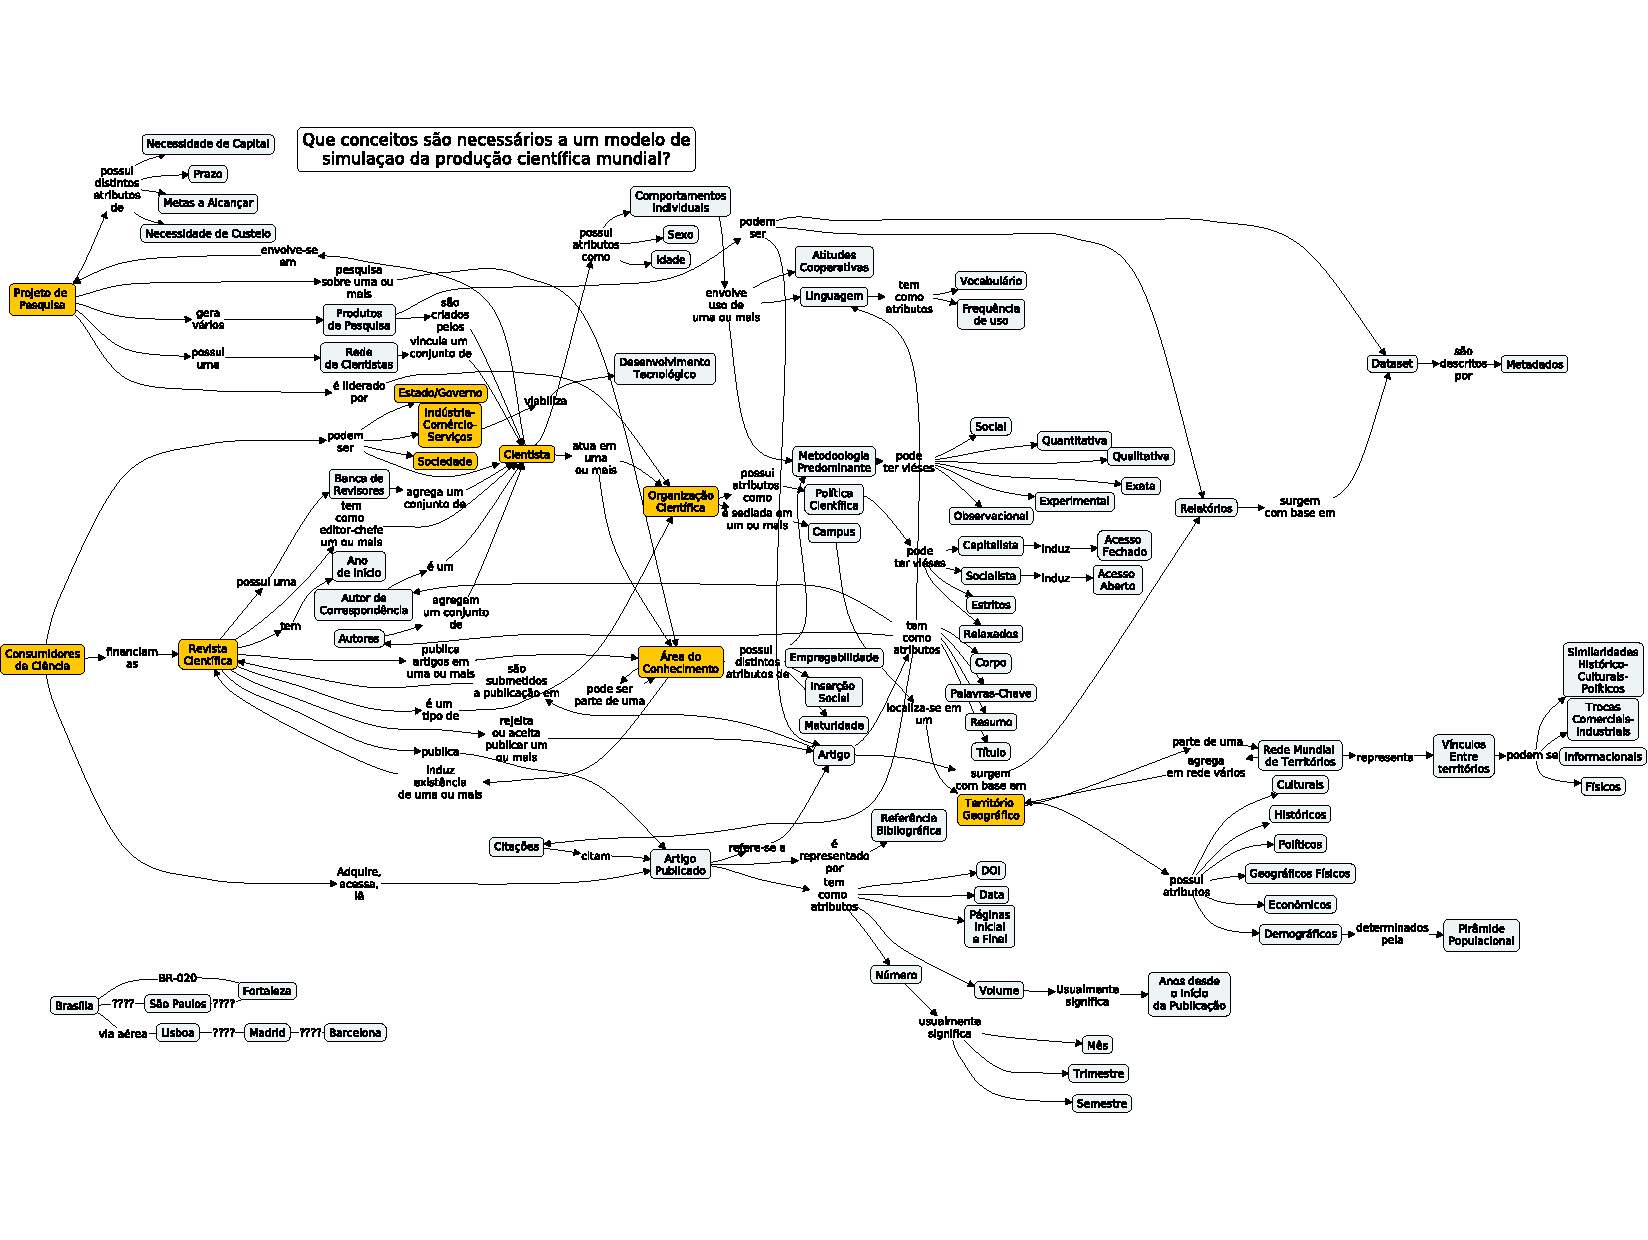
\includegraphics[page=1,angle=90,width=1\textwidth]{aulas/3-Simulacao/CE20211/img/CE20211Conceitos.pdf}
    \caption{Conceitos e atributos centrais da simulação CE20211.}
    \label{fig:CE20211:ConceitosCentrais}
\end{figure}

Os parágrafos a seguir expressam as principais características do modelo, agrupados por temas.

\subsubsection{Sobre Territórios Geográficos} Os territórios são espaços geográficos onde ocorre a produção do conhecimento, e o conhecimento científico produzido em um território geralmente é voltado para a compreensão de problemas que ocorrem nesse território, pois a ciência possui um senso de utilidade, entre outros.
O quadro \ref{tab:ce20211:territorios} apresenta as sentenças centrais sobre a modelagem dos territórios.

\begin{table}
\resizebox{\textwidth}{!}{%
\begin{tabular}{|l|l|l|}
\hline
\textbf{Conceito}           & \textbf{Predicado} & \textbf{Conceito}           \\ \hline
Território Geográfico       & possui atributos   & Culturais                   \\ \hline
Território Geográfico       & possui atributos   & Demográficos                \\ \hline
Território Geográfico       & possui atributos   & Econômicos                  \\ \hline
Território Geográfico       & possui atributos   & Geográficos Físicos         \\ \hline
Território Geográfico       & possui atributos   & Históricos                  \\ \hline
Território Geográfico       & possui atributos   & Políticos                   \\ \hline
Território Geográfico       & é parte de uma     & Rede Mundial de Territórios \\ \hline
Rede Mundial de Territórios & agrega em rede vários & Território Geográfico                         \\ \hline
Rede Mundial de Territórios & representa         & Vínculos Entre territórios  \\ \hline
Vínculos Entre territórios  & podem ser          & Físicos                     \\ \hline
Vínculos Entre territórios  & podem ser          & Informacionais              \\ \hline
Vínculos Entre territórios  & podem ser             & Similaridades Histórico- Culturais- Políticos \\ \hline
Vínculos Entre territórios  & podem ser             & Trocas Comerciais- Industriais                \\ \hline
\end{tabular}%
}
    \caption{Sentenças lógicas sobre Territórios no modelo CE20211.}
    \label{tab:ce20211:territorios}
\end{table}

Com base no quadro \ref{tab:ce20211:territorios}, os agentes do tipo território geográfico possuem uma população (atributo demográfico), que possui comportamentos (cultura), realiza trocas de recursos entre si (economia), uma sequência de fatos importantes, determinantes dos rumos da população e do próprio território (história), uma rede de interesses, onde algumas pessoas assumem papel mais central e outras mais periféricas (política) e que se integram na forma de uma rede (um grafo), que interliga o território e sua população a outros territórios, de forma heterogênea.

A figura \ref{fig:malha} apresenta um exemplo da rede de influência das cidades (territórios) no Brasil, em 2018, produzida pelo IBGE \citep{coordenacao_de_geografia_do_ibge_regioes_2020}.

\begin{figure}
    \framebox{
    \includegraphics[page=1,width=\textwidth,clip=true,trim=1.2cm 2.5cm 2cm 4cm]{aulas/3-Simulacao/CE20211/img/liv101728_p14.pdf}
    }
    \caption{Rede de integração entre os municípios brasileiros, em 2018. Fonte: \cite[p. 14]{coordenacao_de_geografia_do_ibge_regioes_2020}}
    \label{fig:malha}
\end{figure}

A partir da página do \cite{ibge_regioes_2021} é possível se obter um \textit{dataset} contendo dados detalhados de modelagem da rede graficamente apresentada na figura \ref{fig:malha}, de modo a se obter um conjunto de parâmetros de grafo capazes de gerar de forma artificial, uma malha territorial simulada.

\subsection{Escalonamento e Parâmetros}

Os principais parâmetros para o modelo de simulação CE20111 são definidos a partir de respostas quantitativas e algorítmicas a processos, com base na tabela ``Frases de ligação do modelo'' da planilha CE20211.ods.

A sequência de apresentação dos processos segue a lógica de inicialização e escalonamento do modelo.

Em refinamento à sequência de escalonamento do processo, um conjunto de respostas a questões pertinentes a simulação de cada processo, devem ser feitas por grupos de até três alunos, com base no especificado a partir da tarefa 3.4 - elaboração do modelo conceitual.
%(já está aberta) e 3.5 - implementação do algoritmo em Python, a partir do esqueleto da simulação (na semana que vem).
%Na terceira semana, o modelo será integrado e testado.
%Após o modelo integrado e testando serão feitas análises inciais. e uma vez o modelo minimante funcional, cada grupo vai fazer o desenho das experimentações com o modelo implementado.


\begin{description}

\item [Surgem os territórios] 

\item [Surgem as linguagens] 

\item [Surgem as áreas do Conhecimento] 

\item [Surgem as organizações e \textit{campi} nos territórios] 

\item [Cientistas pesquisam em áreas] 

\item [Surgem as revistas científicas]

\item [Cientistas trabalham em organizações] 

\item [Cientistas atuam em área, organização, e  território] 

\item [Surgem os Projetos] 
\item [Cientistas se engajam em projetos] 
\item [Projetos geram Produtos Científicos] 
\item[Cientistas empregam linguagens] 

\item [Cientistas escrevem artigos] 

\item [Cientistas fazem citações em artigos] 

\item [Revisores avaliam artigos submetidos por cientistas]  

\item [Artigos são publicados por revistas] 
\item [Artigos são referenciados] 
\item [Ocorre o consumo da Ciência] 
\end{description}

Para cada um dos processos listados, a seguir é feita uma lista de questões, buscando respostas quantitativas e algorítmicas que serão base para implementar o algoritmo e calibrar o modelo. Cada conjunto de questões apresenta um código (\#1, \#2 etc). Associado a cada conjunto, são feitas recomendações sobre como pode ser feita a busca por informações que indiquem valores para parâmetros e estrutura para algoritmos, usando-se, onde pertinente, esqueleto de codificação na linguagem Python.   

\subsubsection{Surgem os territórios (Questões \#14)}

Qual a estrutura de um conjunto de territórios representantes das principais cidades do mundo, onde ocorre a produção científica? De que maneira representar os atributos sintéticos dos territórios, bem como os vínculos físicos, informacionais, similaridades históricas, culturais, políticas, comerciais, industriais e de serviços entre os territórios? Qual a estrutura e comportamento de um modelo numérico quantitativo e(ou) algorítmico para simular a situação? 

\paragraph{Respostas às questões \#14} podem ser buscadas junto a bases de dados geográficas, tais como OpenStreetMap e GoogleMaps, de alcance mundial. 

Uma fonte de informação mais fácil, apenas sobre a organização das cidades no Brasil, inclusive a estrutura da malha de afinidades entre as cidades, que nada mais é que um grafo, foi desenvolvida pelo \cite{ibge_regioes_2021}. 
A partir da mensuração de parâmetros chave desse grafo, tais como:
\begin{itemize}
    \item distribuição de frequência dos tamanhos dos vértices (usando como tamanho a população das cidades);
    \item peso das arestas do grafo (a partir da intensidade de afinidades interurbanos)
    \item índices de clusterização dos grafos;
    \item índices de centralidade;
    \item e outras medidas de grafos;
\end{itemize} 
podem ser encontrados valores, que inseridos em bibliotecas de geração de grafos, tais como networkx \citep{hagberg_exploring_2008}, poderão criar uma malha territorial artificial.

\paragraph{Essa questão será respondida pelo grupo} Jorge Fernandes

\subsubsection{Surgem as linguagens (Questões \#8)} Quantas linguagens de escrita e publicação de artigos são usadas no mundo? Qual a distribuição de frequência delas? Qual o vocabulário de cada uma delas? Como sintetizar um vocabulário para um conjunto de linguagens a serem usadas na escrita dos artigos? Qual a frequência de uso de cada uma delas? Qual a estrutura e comportamento de um modelo numérico quantitativo e(ou) algorítmico para simular essa situação?

\paragraph{Respostas às questões \#8} tem como ponto de partida a ligação visceral entre linguagem e território, estudada na área de linguística, usando como ponto de partida o trabalho de \cite{magadan_language_2020}.
De outra forma, é importante ter-se uma estimativa da quantidade e distribuição de frequência de uso de linguagens dispersas ao redor do mundo, que pode ser obtida a partir de \cite{infoplease_languages_2021}. 
Por fim, é necessário escolher pelo menos cinco distintas linguagens que podem ser usadas para escrita de artigos, sendo uma predominante, como ocorre hoje com o inglês, e as outras com frequência reduzida, conforme a curva atualmente usada na publicação mundial.
Para sintetizar artificialmente as linguagens e vocabulário de termos a ser usado na escrita de artigos, pode-se usar \cite{vulgarlang_fantasy_2021}.
Durante a construção sintética dos artigos, é preciso oferecer um serviço gerador de sentenças a ser usado pelos autores.

\paragraph{Essa questão será respondida pelo grupo}

\begin{itemize}
    \item - João Pedro Sadéri da Silva - 170126021
    \item - Matheus Arruda Aguiar - 180127659
\end{itemize}

\subsubsection{Surgem as áreas do Conhecimento (Questões \#15)} 
Quantas áreas de conhecimento existem? Como as áreas do conhecimento se organizam hierarquicamente? Qual a forma da distribuição de frequência dessas áreas nas organizações? Nos territórios? Quais as características metodológicas predominantes nessas áreas? Qual a estrutura e comportamento de um modelo numérico quantitativo e(ou) algorítmico para simular a criação das áreas do conhecimento, sua organização hierárquica e sua vinculação aos territórios? 


\paragraph{Respostas às questões \#15} pode ser obtidas a partir da utilização de uma estrutura de organização do conhecimento já existente, e utilizando-se como referências quantitativas e qualitativas a própria estrutura de áreas do conhecimento, programas de pós-graduação e docentes atuantes em pós-graduação, geradas pela CAPES - Coordenação de Acompanhamento de Pessoal de Ensino Superior, agência do Ministério da Educação. 

Para conhecer a hierarquia das áreas do conhecimento veja \cite{capes_tabela_2021}. A partir dessa página, é possível encontra-se a organização do conhecimento usado na pós-graduação brasileira, que apresenta 3 colégios, subdivididos em nove grandes áreas do conhecimento, subdivididos em 49 áreas do conhecimento. Essa organização tem grandes similaridades com o que é usado no mundo inteiro.

Para conhecer as características metodológicas das pesquisas conduzidas nas 49 (quarenta e nove) áreas do conhecimento organizadas pela CAPES, veja os documentos produzidos pelos especialistas referentes à avaliação de cada uma das  \cite{capes_documentos_2018}. Uma vez que trata-se de uma tarefa muito complexa analisar as metodologias de cada uma das áreas de avaliação, considere pertinente avaliar apenas uma área pertencente a cada uma das 9 (nove) grandes áreas, para adotar como base para o restante das áreas.

Para conhecer a complexidade, impacto social e intensidade de pesquisa (quantidade de pesquisadores) conduzida em cada uma das 49 áreas, tome por base:
\begin{description}
    \item [Para estimar a complexidade] use a planilha da situação da pós-graduação brasileira no ano de 2020, em \cite{capes_plataforma_2021} e compare a quantidade de programas em cada área;
    \item [Para estimar a intensidade de pesquisa] use a planilha da quantidade de docentes nas pós-graduações, por área do conhecimento, em \cite{capes_docentes_2020}. 
    \item [Para estimar o impacto social] use a quantidade de bolsas distribuídas em cada uma das 9 grandes áreas, em \cite{capes_geocapes_2021}.
\end{description}

\paragraph{Essa questão será respondida pelo grupo} 
Trio:
\begin{itemize}
    \item João Francisco Gomes Targino - 18/0102991
    \item João Gabriel Ferreira Saraiva - 18/0103016
    \item João Victor Pinheiro de Souza - 18/0103407
\end{itemize}

\subsubsection{Surgem as organizações e \textit{campi} nos territórios (Questões \#11)}
Como as organizações e seus campi são distribuídos nos territórios? Quantos campi cada organização possui? Qual o formato da curva? Distribuição de frequência? Como as características dos territórios influenciam a existência ou não de campi? Qual a estrutura e comportamento de um modelo numérico quantitativo e(ou) algorítmico para simular a situação de criação de organizações, campi e alocação nos territórios?

\paragraph{Respostas às questões \#11}
podem ser obtidas de forma aproximada a partir da comparação entre a população e riqueza dos territórios, e a presença de organizações de ensino que possuem programas de pesquisa neles. Cabe, para obter-se uma estimativa da distribuição das organizações nos territórios, traçar uma correlação entre as cidades brasileiras e  presença dessas organizações com programas de pós-graduação nos municípios brasileiros no ano de 2019, como disponível em \cite{capes_programas_2021}. 

Para identificar a distribuição de organizações em campi, pode-se utilizar o mesmo arquivo para identificar, para cada organização de ensino nas tabelas em  \cite{capes_programas_2021}, a quantidade de municípios em que elas estão presentes, bem como a afinidade por proximidade entre os municípios.

\paragraph{Análise de gráficos relacionados ao tema}
Para o tema "Como surgem as organizações nos territórios", nós procuramos primeiro buscar em quais territórios a produção científica é mais frequente, uma vez que produção científica é indicador de organização científica ativa; depois procuramos quais tipos de organizações produzem mais, e por último buscamos analisar o ritmo de produção com o PIB per capita regional. As fontes para coleta de dados foram escolhidas com base na recomendação inicial do professor e com base numa busca no recurso \textit{https://dados.gov.br/dataset}, em procura de dados relativos aos municípios que dessem um \textit{insight} em porque os campi são distribuídos da forma que são.

A ideia com o primeiro gráfico, produção científica por território, era de termos uma visualização dos territórios nacionais que compunham a maior parte da produção nacional de pesquisa. Nossa suposição era de que os maiores centros urbanos fossem responsáveis pelas maiores quantidades de pesquisa (principalmente por serem as maiores concentrações de pessoas). Como esperado foi encontrado uma correlação entre centros urbanos e maior produção, então pudemos chegar à conclusão de que lugares com maior concentração populacional instigam a criação de centros de pesquisa. 

Em seguida, no gráfico 2, produção científica por tipo de instituição, vemos uma predominância de instituições federais na área de pesquisa brasileira, seguidas por estaduais, privadas e por ultimo municipais. Então é possível concluir que a iniciativa pública (mais de 75\% das produções disponíveis no \textit{dataset}) é agente indispensável para a pesquisa nacional. Isso somado ao fato concluído no primeiro gráfico mostra a necessidade de criação de centros de ensino públicos em lugares com concentração populacional.

E no gráfico 3, PIB per capita por produção científica, nossa expectativa era de encontrar uma relação demonstrando que em lugares com maior PIB, a produção seria mais intensificada. Entretanto o resultado encontrado foi diferente. O gráfico que encontramos mostra uma distribuição relativamente uniforme de produção nos níveis de produção baixa, e nos pontos de produção alta não se encontra relação disso com PIB (os dois pontos com maiores produções estão na média da escala de PIB utilizada). Então não foi possível encontrar correlação entre estes dois valores. Aparenta ocorrer uma correlação positiva fraca entre PIB per capita e produção científica, mas não temos com o \textit{dataset} utilizado dados o suficiente para ter confiança nessa intuição.

\paragraph{Essa questão será respondida pelo grupo} Trio:
\begin{itemize}
    \item Lucas Vinicius ~ 17/0061001
    \item Rafael Gonçalves ~ 17/0043959
    \item Leonardo Rodrigues ~ 17/0060543
\end{itemize}

\subsubsection{Surgem os cientistas, que pesquisam em áreas (Questões \#3)} 
Como surgem os cientistas? Como vem à existência? Que idade, sexo, atitudes comportamentais e outros fatores relevantes eles exibem? Como pode ser criado um modelo numérico quantitativo que indique um número que sumarize os quatro fatores, determinantes da chance de um cientista se interessar por pesquisar numa área de pesquisa específica, em função dos atributos da área de pesquisa, como sua inserção no mercado, relevância social, empregabilidade, maturidade etc? Qual a estrutura e comportamento de um modelo numérico quantitativo e(ou) algorítmico para simular essa situação?

\paragraph{Respostas às questões \#3} pode ser obtidas no arquivo de docentes participantes dos programas de pós-graduação no Brasil, no ano de 2019, como disponível em \cite{capes_docentes_2020}. No ano de 2019 existiam 107.113 docentes vinculados a programas de pós-graduação \textit{Strictu senso} (mestrado e doutorado) no Brasil. As planilhas apresentam entre outros dados, ano de nascimento, área e ano de formação no doutorado e(ou) mestrado, e área de atuação dos mesmos.
Crie, a partir desse dados, um estimador de atitudes (chance de escolher uma área, idade em que atinge o ápice da carreira científica) etc.

\paragraph{Essa questão será respondida pelo grupo} 
\begin{itemize}
    \item Caroline - 16/0067766
    \item Kailany - 17/0147720
\end{itemize}

\subsubsection{Surgem as revistas científicas (Questões \#9)}
Quantas revistas científicas existem? Quantas existem por área do conhecimento? Quantas revistas focam nos problemas existentes em cada território? são distribuições normais,  exponenciais, logarítmicas? Qual a estrutura e comportamento de um modelo numérico quantitativo e(ou) algorítmico para simular essa situação?

\paragraph{Respostas às questões \#9} 
podem ser obtidas por aproximação através da consulta à tabela de classificação de revistas científicas por área de avaliação da CAPES, disponível em \cite{capes_qualis_2016}. Na tabela de qualificação de revistas no ano de 2016 (arquivo 
\texttt{classificações\_publicadas\_todas\_as\_areas\_avaliacao1522078273541.xls}), que contém 131.275 registros, é possível identificar aspectos como:
\begin{itemize}
    \item a quantidade aproximada de revistas científicas em língua inglesa, bem como as revistas em língua portuguesa;  
    \item a qualidade, impacto ou pontuação aproximada das revistas, em cada área do conhecimento (use a maior pontuação) como indicador de qualidade ou atratividade da revista;
    \item as revistas mais importantes para cada área do conhecimento;
    \item uma proporção entre revistas do território (em língua portuguesa) e revistas que tem olhar para fora do território brasileiro (em língua inglesa)
\end{itemize}
Com base nesses números, deve-se criar um serviço de revistas, conforme a probabilidade das mesmas publicarem trabalhos em uma determinada área (ou em duas ou mais áreas).

\paragraph{Essa questão será respondida pelo grupo} 
Dupla:
\begin{itemize}
    \item Caroline - 16/0067766
    \item Kailany - 17/0147720
\end{itemize}

\subsubsection{Cientistas trabalham em organizações (Questões \#12)}
Como os cientistas trabalham por organização científica, no mundo? Como assumem o papel de editor-chefe e revisor numa revista e como isso impacta sua presença na área? Como a distribuição de frequência ocorre? Qual a estrutura e comportamento de um modelo numérico quantitativo e(ou) algorítmico para simular a situação de emprego de cientistas por organizações?

\paragraph{Respostas às questões \#12} pode ser obtidas de forma aproximada no arquivo de docentes participantes dos programas de pós-graduação no Brasil, no ano de 2019, como disponível em \cite{capes_docentes_2020}. No ano de 2019 existiam 107.113 docentes vinculados a programas de pós-graduação \textit{Strictu senso} (mestrado e doutorado) no Brasil. As planilhas apresentam entre outros dados, a organização de ensino e o município eo qual estão filiados.
Crie, a partir desse dados, um estimador de emprego de cientista em organização e campus (chance de trabalhar em uma determinada organização em um determinado campus).
Adicionalmente, a chance de um pesquisador vir a ser editor-chefe ou revisor de uma revista está fortemente correlacionada ao nível de avaliação da organização de pesquisa na qual ele trabalha. Nesse caso, perceba que em \cite{capes_programas_2021} é indicado o nível de avaliação de cada programa, em nota que varia de 3 a 7. Use a nota do programa ao qual o docente está vinculado como sendo um valor que aumenta a chance inicial dele ser convidado a participar como editor de uma revista.

\paragraph{Essa questão será respondida pelo grupo}
Ausente

\subsubsection{Cientistas atuam numa área, numa organização, num território (Questões \#2)}
Como um cientista amadurece e escolhe ou tem oportunidade de ingressar numa área de pesquisa para trabalhar, em uma organização situada em um determinado território, em função de atributos cruzados, pessoais, organizacionais, territoriais e da área do conhecimento atuante? Qual a estrutura e comportamento de um modelo numérico quantitativo e(ou) algorítmico para simular essa situação?

\paragraph{Respostas às questões \#2} podem ser obtidas de forma aproximada a partir do arquivo de docentes participantes dos programas de pós-graduação no Brasil, no ano de 2019, como disponível em \cite{capes_docentes_2020}. No ano de 2019 existiam 107.113 docentes vinculados a programas de pós-graduação \textit{Strictu senso} (mestrado e doutorado) no Brasil. As planilhas apresentam entre outros dados, a formação no cientista doutorado e(ou) mestrado, a atual área de atuação dos mesmos, bem como o país e a sigla da IES (Instituição de Ensino Superior) onde ele foi titulado..
Crie, a partir desse dados, um estimador de atitudes (chance de mudar de área, organização e território) etc.

\paragraph{Essa questão será respondida pelo grupo}


\subsubsection{Surgem os Projetos (Questões \#16)} Como surgem os projetos para pesquisa científica? Como surgem os projetos por área do conhecimento, e por organização, e por território? De que maneira fatores econômicos, políticos, culturais, territoriais, por área do conhecimento, determinam a alocação de recursos que viabilizam ou inviabilizam o surgimento, duração e continuidade de um projeto?

\paragraph{Respostas às questões \#16} podem ser obtidas de forma aproximada fazendo-se uma equiparação entre programas de pós-graduação e projetos de pesquisa. Cada programa de pós-graduação pode ser visto como sendo um projeto de pesquisa, e a nota que os programas apresentam, bem como a quantidade de outros programas que ocupam o mesmo território, são  indicadores de oportunidade econômica para materialização de projetos.
A partir do arquivo dos programas de pós-graduação no Brasil, no ano de 2019, como disponível em \cite{capes_programas_2021} crie um estimador do duração e continuidade de um projeto.

\paragraph{Essa questão será respondida pelo grupo}
\begin{itemize}
    \item Alice da Silva de Lima - 18/0112601
    \item Carlos Eduardo de Oliveira Ribeiro - 18/0099094
    \item Giovana Pinho Garcia - 18/0101374
\end{itemize}

\subsubsection{Cientistas se engajam em projetos (Questões \#6)} Como ocorre o engajamento de cientistas em projetos? Em quantos projetos de pesquisa cada cientista se engaja ao longo do tempo? Quantos cientistas se engajam em cada projeto? Qual a duração dese engajamento, qual a distribuição de frequência desse engajamento? Qual a estrutura e comportamento de um modelo numérico quantitativo e(ou) algorítmico para simular essa situação?

\paragraph{Respostas às questões \#6} podem ser obtidas de forma aproximada fazendo-se uma equiparação entre programas de pós-graduação e projetos de pesquisa. Cada programa de pós-graduação pode ser visto como sendo um projeto de pesquisa, e a rede de colaborações de autoria que os membros dos programas de pós-graduação desenvolvem representam, de forma aproximada, o conjunto total de todas as redes de relacionamento presentes em todos os  projetos realizados na organização. Os cientistas com maior centralidade na rede, e que atuam na área ou próximo dela, são os que tem mais chances de serem os coordenadores dos projetos. Os demais cientistas da mesma organização, atuantes na mesma área do projeto, agregam-se à rede do projeto em posições subordinadas ao coordenador.
Com base nas orientações, crie um gerador de engajamento de cientistas em um projeto criado numa organização, campi/território, e área do conhecimento.

\paragraph{Essa questão será respondida pelo grupo} 
Trio:
\begin{itemize}
    \item Henrique - 17/0012280
    \item Luthiery - 17/0040631
    \item Thales - 17/0045919
\end{itemize}


\subsubsection{Projetos geram Produtos Científicos (Questões \#17)} Como os cientistas, engajados em redes nos projetos, em uma ou mais organizações envolvidas, em uma ou mais áreas do conhecimento envolvidas, em um ou mais territórios envolvidos, com limitações maiores ou menores nos recursos alocados, geram os \textit{datasets} e relatórios típicos de um projeto? Os projetos podem fracassar na geração de seus produtos? Qual a estrutura e comportamento de um modelo numérico quantitativo e(ou) algorítmico para simular essa situação? 

\paragraph{Respostas às questões \#17} 
podem ser obtidas a partir de uma fórmula heurística que estime a chance de um projeto ser interrompido, de produzir um dataset, de produzir um relatório, com base nos seguintes princípios:
\begin{itemize}
    \item A chance de um projeto ser interrompido está diretamente ligada ao valor de recursos envolvidos com o projeto, e à qualificação de seu coordenador e equipe.
    \item a chance de um projeto ativo (não interrompido) gerar um dataset está ligado ao valor de recursos envolvidos com o projeto, à qualificação de seu coordenador e equipe, combinados com o viés da metodologia da área de pesquisa envolvida, se mais quantitativo (mais dados) ou mais qualitativo (menos dados);
    \item a chance de um projeto ativo (não interrompido) gerar um relatório está ligada à disponibilidade e riqueza de datasets, ao valor de recursos envolvidos com o projeto, à qualificação de seu coordenador e equipe;
\end{itemize}

Os parâmetros quantitativos de volume e (ou) quantidade de produtos (datasets e relatórios) também deve ser calibrada com base na taxa de produtividade por área de conhecimento, que pode ser estimada com base nos Detalhes da Produção Intelectual Bibliográfica de Programas de Pós-Graduação Stricto Sensu no Brasil [2013 a 2016] \cite{capes_detalhes_2017}.

\paragraph{Essa questão será respondida pelo grupo}
Ausente

\subsubsection{Cientistas empregam linguagens (Questões \#1)}
Como - e de que forma quantitativa - ocorre o emprego de uma ou mais linguagens (no mundo real, português, inglês, francês etc), na escrita de um artigo científico pelos cientistas autores? Como essa escolha ou limitação afeta a chance de sucesso de publicações desse artigo em uma revista cientifica? Como o critério de linguagem de publicação afeta o desempenho de uma revista? Como o uso de uma linguagem afeta a difusão de conhecimento gerado (artigo escrito) naquela linguagem? Qual a estrutura e comportamento de um modelo numérico quantitativo e(ou) algorítmico para simular essa situação?

\paragraph{Respostas às questões \#1} podem ter como ponto de partida conceitual a discussão conduzida por \cite{ramirez-castaneda_disadvantages_2020}, sobre as desvantagens pelas quais passam os pesquisadores que não tem o inglês como língua materna. As referências citadas nesse artigo permitem maior aprofundamento. Em especial, o livro de \cite{gordin_scientific_2015} apresenta em contraponto, um conjunto de argumentos favoráveis à dominação do inglês como língua científica mundial.
Assim sendo, os responsáveis por responder a essa pergunta devem modelar de forma algorítmica e quantitativa a dificuldade que um cientista que não fala inglês tem para escrever um artigo de boa qualidade em inglês.

\paragraph{Essa questão será respondida pelo grupo}
Ausente

\subsubsection{Cientistas escrevem artigos (Questões \#5)} De que forma os cientistas são estimulados, durante os projetos ou após o término dos projetos, a escrever os artigos científicos que darão visibilidade ao conhecimento gerado nos projetos?  Como pode ser sintetizada a escrita de um artigo científico (ainda não publicado), a partir de um ou mais relatórios e dados (\textit{datasets}) de pesquisa? Qual a estrutura e comportamento de um modelo numérico quantitativo e(ou) algorítmico para simular essa situação de escrita de um artigo, sabendo-se que um artigo é escrito baseado na existência de um relatório científico, que possui um conjunto de autores, onde o título, resumo, corpo do texto, e palavras-chave são escritos no vocabulário de uma linguagem específica, e que poderá ou não vir a ser publicado?

\paragraph{Respostas às questões \#5} podem ter seu fundamento prático embasado no trabalho de \cite{gu_developing_2019}, que realizou uma análise de cluster de padrões de publicações de acadêmicos, e gerou uma tipologia de pesquisadores baseada em seis tipos, com as seguintes frequências:
\begin{description}
    \item [singleton] (8\%); 
    \item [small‐team low performer] (16\%)
    \item [small‐team high performer] (17\%);
    \item [big‐team strategist] (22\%)
    \item [free‐style follower] (21\%); e
    \item [life‐time warrior] (17\%)
\end{description}
Com base na leitura desse artigo, e na compreensão dos determinantes gerados pelos atributos dos pesquisadores analisados, construa um estimador da chance de um membro qualquer do projeto, escrever um artigo, em co-autoria com os demais. O seu modelo também deve considerar que são poucas as chances de escrita, se não houverem produtos subjacentes, especialmente relatórios, mas também os datasets no projeto.
Uma vez que o artigo seja escrito por um ou mais autores, ele deve conter um título, resumo e palavras-chave, que serão usados no processo de criação da referência bibliográfica e indexação.

\paragraph{Essa questão será respondida pelo grupo} 
Dupla:
\begin{itemize}
    \item Gabriel Nazareno Halabi - 15/0010290
    \item Paulo Maurício Costa Lopes - 18/0112520
\end{itemize}

\subsubsection{Cientistas fazem citações em artigos (Questões \#7)} Qual a estrutura e comportamento numérico das citações que um artigo faz durante sua escrita? Quantas citações cada artigo faz? Como ocorre a distribuição de frequência nas citações? Como os artigos são escolhidos para serem citados? Como sintetizar esse processo de citação? Qual a estrutura e comportamento de um modelo numérico quantitativo e(ou) algorítmico para simular essa situação?

\paragraph{Respostas às questões \#7} deve ser elaboradas a partir do estudo do padrão de citações presente em bases de dados bibliográficas com citações, geradas na Web of Science ou SCOPUS, como a disponível em  \texttt{experiments / jhcf / PesquisaBibliogr / Computacao Experimental / WoS-20210803 / 8155recs.txt}. A partir desse dataset devem ser geradas as distribuições de frequência de citações por artigo. Já acerca dos artigos citados, podem ser citados apenas artigos já publicados e \textbf{referenciados}, e dessa forma, os primeiros artigos da simulação terão nenhuma, ou poucas citações, obtendo uma situação de \textit{steady-state} após um período de milhares de publicações. Observe que as referências aos artigos são essenciais para que eles possam ser encontrados e lidos.

\paragraph{Essa questão será respondida pelo grupo}

\begin{itemize}
 \item Vitor Vasconcelos de Oliveira - 18/0114778
 \item Álvaro Veloso Cavalcanti Luz - 18/0115391 
 \item Gabriel Cesário Silva Martins - 18/0100912 
\end{itemize}


\subsubsection{Revisores avaliam artigos submetidos por cientistas (Questões \#13)}  Como os cientistas escolhem as revistas para submeter à publicação? Quais fatores determinam suas preferências? Como os revisores das revistas avaliam os artigos submetidos à publicação pelos seus cientistas pares? Quantos revisores existem em cada \textit{scientific journal}? Como ocorre essa distribuição de frequência? Quais as taxas de rejeição ou aceitação de artigos por revisor? Quanto tempo os revisores passar para avaliar um artigo? Que critérios são usados para aceitar ou rejeitar artigos? Quantos dias leva para ser tomada a decisão de aceitação ou rejeição? Qual a taxa de rejeição de artigos por revista e por área? Qual a estrutura e comportamento de um modelo numérico quantitativo e(ou) algorítmico para simular a situação? 

\paragraph{Respostas às questões \#13} devem se fundamentar nas questões teóricas que são subjacentes ao uso da revisão por pares na publicação científica. O trabalho de \cite{kovanis_evaluating_2017} apresenta um excelente discussão sobre a questão.
A partir de uma leitura rápida desse artigo, e de outros, desenvolva um estimador da chance de um artigo ser aprovado ou rejeitado considerando o que é encaminhado pelos três revisores que usualmente avaliam um artigo submetido a uma revista, em um período de tempo de algumas semanas. Observe que a distribuição do artigo pelos revisores é feita por afinidade da área do artigo com a área de atuação do revisor, o que pode envolver também a questão da afinidade do território entre os autores e o revisor. A chance de submissão de um artigo a uma revista aumenta conforme aumentam os índices-H das revistas, inicialmente zerados. Investigue também as taxas médias de rejeição a artigos, estimando faixas de rejeição, que vão crescendo à medida em que os índices-H da revista vão também crescendo, bem como vão crescendo se cresce a fila de artigos aceitos e ainda não publicados.

\paragraph{Essa questão será respondida pelo grupo}
Ausente

\subsubsection{Artigos são publicados por revistas (Questões \#10)} Quantos artigos são publicados por cada revista, a cada número e volume? Quantos volumes por ano? Quais as formas das distribuições de frequência? Qual a estrutura e comportamento de um modelo numérico quantitativo e(ou) algorítmico para simular essa situação?

\paragraph{Respostas às questões \#10} devem se fundamentar na disponibilidade que as revistas tem para publicar artigos. Toda revista tem pelo menos cinco filas de artigos:
\begin{itemize}
    \item Uma fila de artigos submetidos a serem avaliados;
    \item Uma fila de artigos em avaliação;
    \item Uma fila de artigos rejeitados;
    \item Uma fila de artigos aceitos;
    \item uma fila de artigos publicados;
\end{itemize} 
As revistas possuem recursos limitados de avaliadores, que só conseguem avaliar um número máximo de artigos numa taxa de tempo, bem como uma fila de artigos publicados que também só publica x artigos por numero por volume ao longo de um ano.
Os artigos rejeitados podem ser submetidos pelos seus autores a outras revistas. Os aceitos para publicação tem que aguardar na fila o momento de serem publicados, até que se atinja um equilíbrio entre submissão, rejeição/aceitação e publicação. O modelo a ser desenvolvido deve equilibrar essas questões, dentro de parâmetros próximos aos valores reais praticados por revistas. Sugere-se uma investigação em três revistas reais, uma de alto desempenho e impacto, uma de médio e uma de baixo, para estimar os parâmetros da simulação.  

\paragraph{Essa questão será respondida pelo grupo}
Ausente

\subsubsection{Artigos são referenciados (Questões \#4)} Como pode ser sintetizada a referenciação e inexação de um artigo, em uma referência bibliográfica? Qual a estrutura e comportamento de um modelo numérico quantitativo e(ou) algorítmico para simular essa situação sabendo-se que um artigo publicado em uma revista científica é representado por uma referência bibliográfica contendo data de publicação, DOI, ano, volume e número, páginas inicial e final, autor de correspondência, além dos atributos inerentes ao artigo? Será que todos os artigos são indexados de forma equivalente, independentemente da linguagem e território vinculados? Qual a estrutura e comportamento de um modelo numérico quantitativo e(ou) algorítmico para simular essa situação?

\paragraph{Respostas às questões \#4} devem se fundamentar no fato de que o consumo da ciência ocorre por meio do acesso aos registros bibliográficos que são produzidos pelos sistemas de indexação, como Web of Science, Scopus e Google Scholar. Após ler o trabalho de \cite{gusenbauer_google_2019} desenvolva um pelo menos três diferentes agentes indexadores dos artigos, que com uma certa taxa de sucesso, maior ou menor, visita as revistas e gera registros bibliográficos no formato BIBTEX, que serão disponibilizados para busca, recuperação e leitura pelos consumidores da ciência.

\paragraph{Essa questão será respondida pelo grupo}
Ausente

\subsubsection{Ocorre o consumo da ciência (Questões \#18)}
Quem consome os produtos essenciais da ciência, os artigos científicos publicados? De que modo ocorre o consumo de produtos científicos pelos Estados e Governos? Pela Indústria, Comércio e Serviços? Pela Sociedade em geral? Pelos próprios cientistas? Como o consumo varia por área do conhecimento, território, visibilidade da revista? e como esse consumo determina a disponibilidade de recursos para o ciclo de vida do sistema de organizações, revistas, projetos, cientistas e áreas do conhecimento? 

\paragraph{Respostas às questões \#18} dependem da compreensão de que:
\begin{itemize}
    \item O Estado/Governo consome ciência para elaborar melhores políticas públicas, de ordem econômica, social, ambiental, educacional, de saúde, de segurança e defesa etc. O maior ou menor nível de organização política de um Estado/Governo é determinante do maior ou menor nível de consumo de ciência pelo Estado, e consequentemente o maior ou menor aporte de dinheiro para o funcionamento das organizações científicas daquele território;
    \item O setor privado consome ciência para desenvolver tecnologia, a fim de melhorar indústria, comércio e serviços. Se a ciência é produzida para fora do território, há menor interesse privado no consumo da ciência, pois ela não será útil para a solução dos problemas. Nesse caso, não terão interesse em estimular o aporte do governo na ciência.
\end{itemize}
Com base nessa compreensão, você deve fazer a leitura do artigo de \cite{schepelmann_evidence-based_2021}, para desenvolver melhor percepção da questão, e desenvolver uma abordagem na qual cada território atua como agente do Estado/Governo e setor Privado, investindo recursos na promoção de pesquisas junto às organizações de pesquisa presentes no seu território, ou próximas a ele.  

\paragraph{Essa questão será respondida pelo grupo}
\begin{itemize}
    \item José Fortes Neto - 160128331
    \item Adelson Jhonata Silva de Sousa - 180114913
    \item Heitor de Lima Belém - 160123950
\end{itemize}

\subsection{Conceitos no Design da Simulação da Produção Mundial da Ciência}


\subsection{Detalhes da Simulação da Produção Mundial da Ciência}

\subsubsection{Submodelos}

\paragraph{Como surgem os territórios? por Jorge H c Fernandes}

Os parâmetros matemáticos, estatísticos e computacionais necessários ao refinamento deste submodelo da simulação são sumarizados no apêndice \ref{surgeosterritorios} deste documento.

A análise é gerada por meio do notebook R Markdown, 
%a seguir listado.
%\lstinputlisting[language=R]{
em \url{experiments/jhcf/ProducaoDaCiencia/R/Territorios/ComoSurgemOsTerritorios.Rmd}


\paragraph{Surgem as Linguagens Por João Pedro Sadéri da Silva e Matheus Arruda Aguiar}

Os parâmetros matemáticos, estatísticos e computacionais necessários ao refinamento desse submodelo de simulação são sumarizados no apêndice \ref{surgemaslinguagens} deste documento.

A análise é gerada por meio do notebook R Markdown, em \url{experiments/jpsaderi/ProducaoDaCiencia/R/Linguagens/SurgeAsLinguagens.Rmd}

\paragraph{Consumo e Investimentos na Ciência Por Adelson Jhonata Silva de Sousa, Heitor de Lima Belém e José Fortes Neto}

Os parâmetros matemáticos, estatísticos e computacionais necessários ao refinamento desse submodelo de simulação são sumarizados no apêndice \ref{investimentoCiencia} deste documento.

A análise é gerada por meio do notebook R Markdown, em \url{experiments/jhonatasousa58/PesquisaDaCiencia/investimentoCiencia.Rmd}

\paragraph{Como surgem as áreas do conhecimento Por João Gabriel Ferreira Saraiva, João Francisco Gomes Targino e João Victor Pinheiro de Souza}

Os parâmetros matemáticos, estatísticos e computacionais necessários ao refinamento desse submodelo de simulação são sumarizados no apêndice \ref{SurgemAreas} deste documento.

A análise é gerada por meio do notebook R Markdown, em \url{experiments/Joaofsrs/AreasDoConhecimento/R/Areas_Conhecimento.Rmd}
